% Options for packages loaded elsewhere
\PassOptionsToPackage{unicode}{hyperref}
\PassOptionsToPackage{hyphens}{url}
%
\documentclass[
]{article}
\usepackage{amsmath,amssymb}
\usepackage{iftex}
\ifPDFTeX
  \usepackage[T1]{fontenc}
  \usepackage[utf8]{inputenc}
  \usepackage{textcomp} % provide euro and other symbols
\else % if luatex or xetex
  \usepackage{unicode-math} % this also loads fontspec
  \defaultfontfeatures{Scale=MatchLowercase}
  \defaultfontfeatures[\rmfamily]{Ligatures=TeX,Scale=1}
\fi
\usepackage{lmodern}
\ifPDFTeX\else
  % xetex/luatex font selection
\fi
% Use upquote if available, for straight quotes in verbatim environments
\IfFileExists{upquote.sty}{\usepackage{upquote}}{}
\IfFileExists{microtype.sty}{% use microtype if available
  \usepackage[]{microtype}
  \UseMicrotypeSet[protrusion]{basicmath} % disable protrusion for tt fonts
}{}
\makeatletter
\@ifundefined{KOMAClassName}{% if non-KOMA class
  \IfFileExists{parskip.sty}{%
    \usepackage{parskip}
  }{% else
    \setlength{\parindent}{0pt}
    \setlength{\parskip}{6pt plus 2pt minus 1pt}}
}{% if KOMA class
  \KOMAoptions{parskip=half}}
\makeatother
\usepackage{xcolor}
\usepackage[margin=1in]{geometry}
\usepackage{graphicx}
\makeatletter
\def\maxwidth{\ifdim\Gin@nat@width>\linewidth\linewidth\else\Gin@nat@width\fi}
\def\maxheight{\ifdim\Gin@nat@height>\textheight\textheight\else\Gin@nat@height\fi}
\makeatother
% Scale images if necessary, so that they will not overflow the page
% margins by default, and it is still possible to overwrite the defaults
% using explicit options in \includegraphics[width, height, ...]{}
\setkeys{Gin}{width=\maxwidth,height=\maxheight,keepaspectratio}
% Set default figure placement to htbp
\makeatletter
\def\fps@figure{htbp}
\makeatother
\setlength{\emergencystretch}{3em} % prevent overfull lines
\providecommand{\tightlist}{%
  \setlength{\itemsep}{0pt}\setlength{\parskip}{0pt}}
\setcounter{secnumdepth}{5}
\usepackage[german]{babel}
\usepackage{mathtools}
\usepackage{tikz}
\usepackage{pgf}
\usepackage{csquotes}
\AtBeginDocument{
\renewcommand{\maketitle}{}
}
\PassOptionsToPackage{a4paper,margin = 2.5cm}{geometry}
\usepackage{geometry}
\usepackage{float}
\newcommand{\bcenter}{\begin{center}}
\newcommand{\ecenter}{\end{center}}
\renewcommand{\contentsname}{Inhalt}
\usepackage{blindtext}
\usepackage[backend=biber, style = apa]{biblatex}
\addbibresource{Literatur.bib}
\ifLuaTeX
  \usepackage{selnolig}  % disable illegal ligatures
\fi
\usepackage[]{biblatex}
\addbibresource{Literatur.bib}
\IfFileExists{bookmark.sty}{\usepackage{bookmark}}{\usepackage{hyperref}}
\IfFileExists{xurl.sty}{\usepackage{xurl}}{} % add URL line breaks if available
\urlstyle{same}
\hypersetup{
  pdftitle={Funktionsweise},
  pdfauthor={Franz Andersch \& Niklas Münz},
  hidelinks,
  pdfcreator={LaTeX via pandoc}}

\title{Funktionsweise}
\author{Franz Andersch \& Niklas Münz}
\date{2024-08-29}

\begin{document}
\maketitle

\subsection{Hard Margin Classifier}

Um das grundlegende Prinzip der \textit{SVM} darzustellen, gehen wir
zuerst von einer Datensituation aus, in der sich zwei Gruppen optimal
durch eine lineare Entscheidungsgrenze trennen lassen. Das endgültige
Ziel ist es eine sogenannte Hyperplane zu finden die diese Daten
möglichst gut separiert und als Entscheidungsgrenze funktioniert. Die
allgemeine Form einer solchen Hyperplane lautet \begin{align}
\beta_0+ \beta_1 X_1+\beta_2 X_2+...+\beta_n X_n=0\label{eq:hyperebene}
\end{align} oder in Vektorschreibweise \begin{align}
\overline{\beta}\cdot\overline{x}+\beta_0=0 \label{eq:hyperplanevec}
\end{align} Die geometrische Interpretation des Vektors \(\beta\) und
des Skalars \(\beta_0\) wird in Abbildung \ref{fig:Ebene} im
zweidimensionalen Fall dargestellt.

\begin{figure}[htb]
    \centering
    \begin{minipage}{0.45\textwidth} 
        \centering
        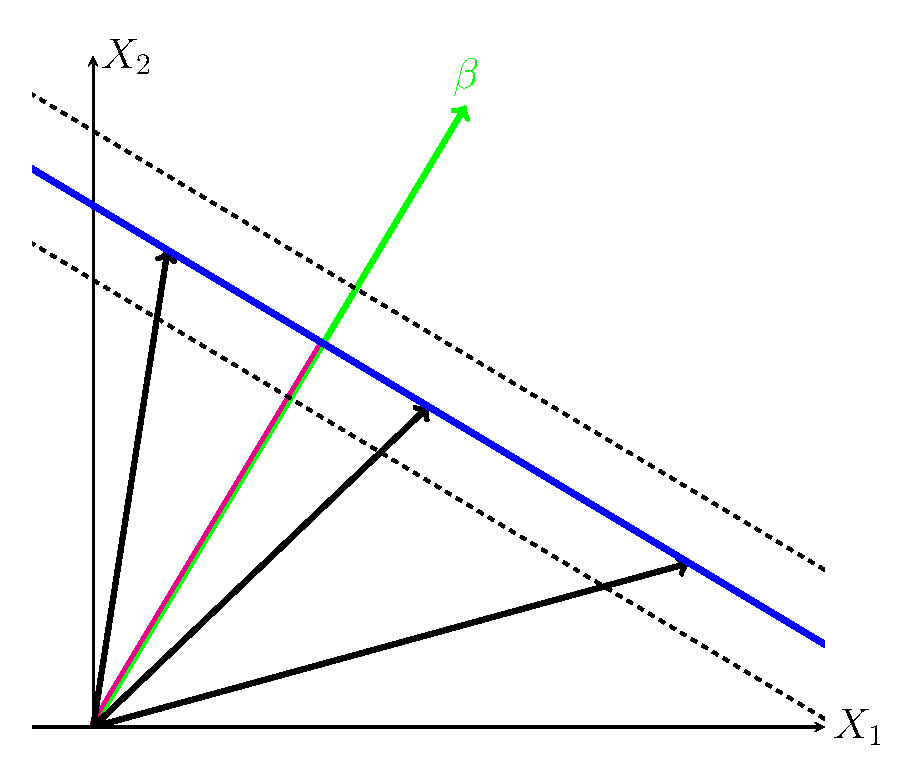
\includegraphics[width=\textwidth,trim=0.5cm 0.5cm 0.5cm 0.5cm]{Images/decision_boundary.pdf} 
        \caption{Konstruktion der Hyperebene}
        \label{fig:Ebene}
    \end{minipage}\hfill
    \begin{minipage}{0.45\textwidth} 
        \centering
        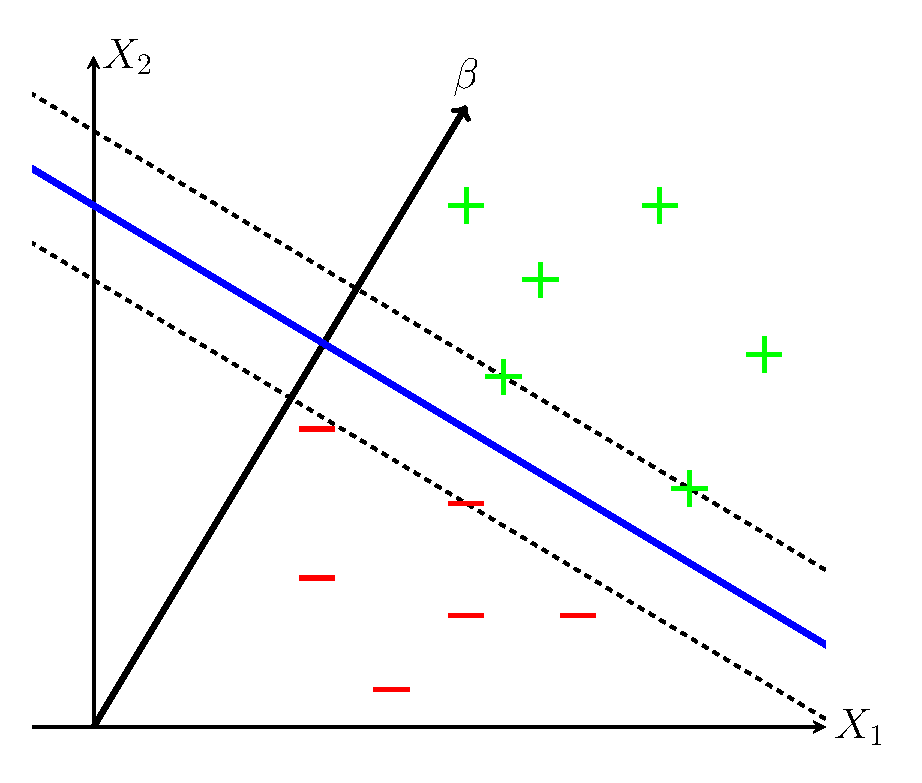
\includegraphics[width=\textwidth,trim=0.5cm 0.5cm 0.5cm 0.5cm]{Images/guttes.pdf}
        \caption{Konstruktion der Margins}
        \label{fig:Margin}
    \end{minipage}
\end{figure}

Die blaue Linie soll die Hyperplane darstellen. Im zweidimensionalen
handelt es sich hier um eine Linie. Der \(2 \times 1\) Vektor
\(\overline{\beta}\) liegt immer senkrecht zur konstruierten Hyperplane.
Würde man alle Vektoren, die auf der Hyperplane landen, auf den
normierten \(\overline{\beta}\)-Vektor projizieren, dann erhält man für
alle diese Projektionen denselben Wert \(c\). Also gilt für alle Punkte,
die auf der Ebene liegen. \begin{align}
\frac{\overline \beta}{||\overline{\beta}||}\cdot \overline{x}=c \Leftrightarrow \overline{\beta}\cdot \overline{x}=c \cdot ||\overline{\beta}||\label{eq:betanull}
\end{align} Ersetzt man in \eqref{eq:betanull}
\(c \cdot ||\overline{\beta}||\) mit \(-\beta_0\) und zieht dies dann
auf die andere Seite, kommt man wieder bei der ursprünglichen Form aus
Formel \eqref{eq:hyperplanevec} raus
\parencite{mavroforakisGeometricApproachSupport2006}.

Als Nächstes stellt sich jetzt die Frage, welches \(\overline{\beta}\)
und \(\beta_0\) die optimale Hyperplane darstellen. Betrachtet man die
Abbildung \ref{fig:Margin}, dann ist zu erkennen, dass die Datenpunkte
durch die blaue Linie getrennt werden. Allerdings könnte man theoretisch
unendlich viele andere Hyperplanes durch Rotation oder Verschiebung
konstruieren, die trotzdem die Daten in ihren Ausprägungen trennen. Um
eine eindeutige Lösung zu finden, wird zunächst ein Bereich um die
Hyperplane abgesteckt. In Abbildung \ref{fig:Margin} dargestellt durch
die gestrichelten schwarzen Linien, welche man als Schranken bezeichnen
könnte. In diesem Bereich sollen keine Datenpunkte liegen, die Schranken
sollen immer parallel zur Hyperplane sein und den gleichen Abstand zu
ihr haben. Außerdem dürfen keine positiven Samples unterhalb der oberen
Schranke liegen und keine negativen oberhalb. Das Gegenteil gilt
dementsprechend für die untere Schranke. Als Definition für die beiden
Schranken wird festgelegt \begin{align}
\overline{\beta}\cdot \overline{x}+\beta_0=1\label{eq:posSV}
\end{align} für die Schranke in Richtung der grünen Datenpunkte und
\begin{align}
\overline{\beta}\cdot \overline{x}+\beta_0=-1\label{eq:negSV}
\end{align} für die Schranke in Richtung der roten Datenpunkte. Aus
dieser Beschränkung für die Hyperplane können wir auch ableiten, dass
für die positiven Samples \(\overline{x}^+\) immer gilt
\(\overline{\beta}\cdot \overline{x}^++\beta_0\ge 1\) und für negative
Samples \(\overline{x}^-\) immer gilt
\(\overline{\beta}\cdot \overline{x}^-+\beta_0\le -1\). Durch das
Einführen einer weiteren Variable \(y\), welche die Eigenschaft hat,
dass sie den Wert 1 bei einem positiven und den Wert -1 bei einem
negativen Sample annimmt, können diese zwei Beschränkungen zu Einer
zusammengefasst werden \parencite{cortesSupportvectorNetworks1995}.
\begin{align}
y_i(\overline{\beta}\cdot \overline{x}_i+\beta_0)\ge 1\label{eq:Nebenbedingung}
\end{align} Da das Verfahren auch \textit{Maximal Margin Classifier}
gennant wird, gilt es jetzt noch eine Definition für den Margin also den
Abstand zwischen den zwei Schranken zu finden, der letztendlich
maximiert werden soll. Damit diese Schranken, maximal weit auseinander
liegen, muss es zwangsläufig Datenpunkte geben, die genau auf den
Schranken liegen. Diese Datenpunkte haben eine wichtige Rolle für die
Konstruktion des Margins. Es sind ausschließlich diese Datenpunkte, die
einen Einfluss auf die finalen Werte von \(\overline{\beta}\) und
\(\beta_0\) haben werden. Sie werden \textit{Support-Vektoren} genannt
und geben den \textit{SVM} ihren Namen.

\begin{figure}[htb]
\centering
 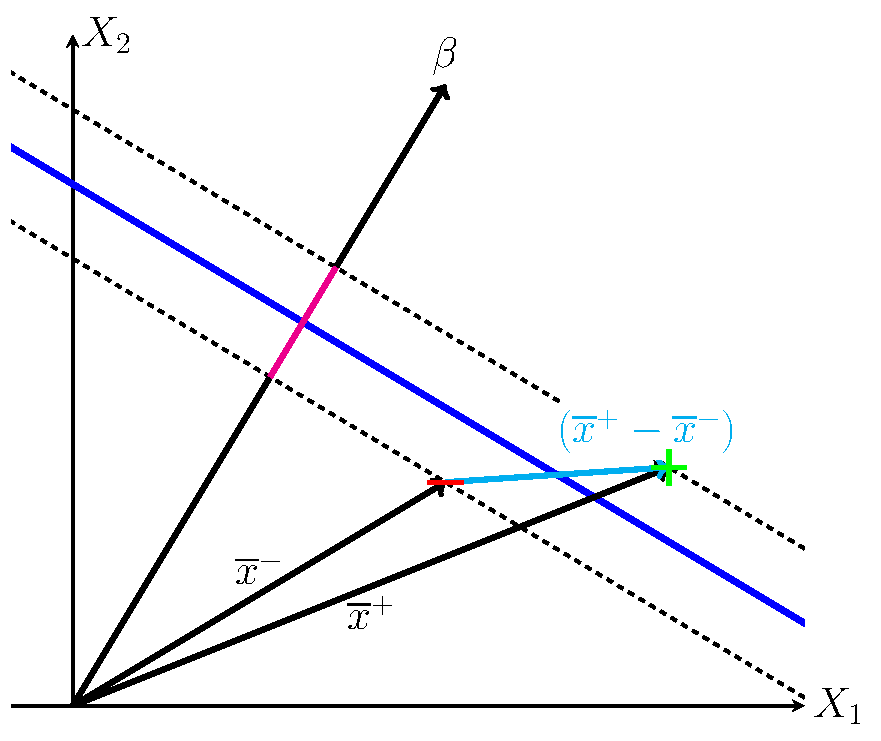
\includegraphics[width=0.5\textwidth,trim=0.5cm 0.5cm 0.5cm 0.5cm]{Images/margin.pdf} 
        \caption{Abhängigkeit des Margins von den Support-Vektoren}
        \label{fig:SupVecs}
\end{figure}

In Abbildung \ref{fig:SupVecs} sind zwei solcher Support-Vektoren zu
einem negativen und positiven Sample dargestellt. Der Margin kann dann
dargestellt werden als eine Projektion dieser Differenz
(\(\overline{x}^+-\overline{x}^+\)) auf den \(\overline{\beta}\)-Vektor.
Damit am Ende die Länge dieses Margins \(M\) herauskommt, muss
\(\overline{\beta}\) noch durch seine Länge geteilt werden.
\begin{align}
M=\frac{\overline{\beta}}{||\overline{\beta}||}\cdot \left(\overline{x}^+-\overline{x}^+\right)=\frac{\overline{\beta}\cdot\overline{x}^- -\overline{\beta}\cdot\overline{x}^+}{||\overline{\beta}||}\label{eq:maring1}
\end{align} Es ist bekannt, dass für positive Support-Vektoren gilt
\(\overline\beta \overline{x}^+ +\beta_0 = 1 \Leftrightarrow \overline\beta \overline{x}^+=1-\beta_0\)
und für negative
\(\overline\beta \overline{x}^- +\beta_0 = -1 \Leftrightarrow \overline\beta \overline{x}^-=-1-\beta_0\).
Setzt man dies ein in \eqref{eq:maring1}, erhält man als
Maximierungsziel \begin{align}
M=\frac{1-\beta_0-(-1-\beta_0)}{||\overline\beta||}=\frac{2}{||\overline\beta||}\label{eq:margin2}
\end{align} Um diesen Maximierungsschritt angenehmer zu gestalten, wird
an der Stelle versucht den Ausdruck
\(\frac{1}{2}||\overline \beta||^2=\frac{1}{2}\overline \beta '\cdot \overline \beta\)
zu minimieren. Was im Endeffekt ebenfalls dazu führt, dass der Ausdruck
in \eqref{eq:margin2} maximiert wird.

Dieses Optimierungsproblem mit der Nebenbedingung aus Formel
\eqref{eq:Nebenbedingung} lässt sich am besten über Lagrange-Multiplier
lösen \begin{align}
\mathcal{L}(\overline\beta,\beta_0,\overline \alpha)=\frac{1}{2}\overline \beta ' \overline \beta-\sum \alpha_i[y_i(\overline \beta \cdot \overline{x_i}+\beta_0)-1]\label{eq:Lagrange}
\end{align} wobei hier \(\overline{\beta}\) und \(\beta_0\) minimiert
und \(\overline{\alpha}\) maximiert wird
\parencite{vapnikEstimationDependencesBased2006}. Wird dieser Ausdruck
partiell abgeleitet und gleich null gesetzt erhält man als
Zwischenergebnis \begin{align}
\frac{\partial \mathcal{L}}{\partial \beta}=\beta-\sum \alpha_i y_i \overline{x_i}\overset{!}{=}0 \Rightarrow \beta=\sum \alpha_i y_i \overline{x_i}\label{eq:solutbeta}
\end{align} Somit zeigt sich, dass \(\overline{\beta}\) als
Linearkombination der Inputvektoren dargestellt werden kann. Weiterhin
gilt für \(\beta_0\) \begin{align}
\frac{\partial \mathcal{L}}{\partial \beta_0}=\sum \alpha_i y_i \overline{x_i}\overset{!}{=}0\label{eq:solutbeta0}
\end{align} Setzt man dies in \eqref{eq:Lagrange} ein erhält man einen
neuen Ausdruck, denn es gilt zu minimieren \begin{align}
\mathcal{L}(\overline \alpha)=-\frac{1}{2}\sum \sum \alpha_i \alpha_j y_i y_j \overline{x}_i \cdot \overline{x}_j+\sum \alpha_i\label{eq:dualproblem}
\end{align} Die Lösung für diesen Ausdruck erfolgt dann über sogenannte
\enquote{standard non linear optimization algorithms for quadratic forms}
\parencite{boserTrainingAlgorithmOptimal1992}. Nachdem für
\(\overline \alpha\) gelöst wurde, kann dies in \eqref{eq:solutbeta}
eingesetzt werden, um das optimale \(\overline{\beta}\) zu erhalten. Es
kann gezeigt werden, dass die gelösten \(\alpha_i\) lediglich für die
Support-Vektoren Werte ungleich Null annehmen. Somit ist der
Koeffizientenvektor \(\overline{\beta}\) sogar eine Linearkombination
von nur den Support-Vektoren
\parencite{boserTrainingAlgorithmOptimal1992}. Die letzte unbekannte
\(\beta_0\) kann gelöst werden, indem man mithilfe von einem
positiven/negativen Support Vektor \eqref{eq:posSV}/ \eqref{eq:negSV}
nach \(\beta_0\) löst.

Mit den gelösten Werten zur optimalen Hyperplane kann jetzt auch eine
Entscheidungsregel für ungelabelte Datenvektoren \(\overline{x}_u\)
konstruiert werden. Bedenkt man also, wenn man einen Vektor, der nicht
auf der Hypeplane liegt in \eqref{eq:betanull} einsetzt, erhält man also
\(\frac{\overline \beta}{||\overline{\beta}||}\cdot \overline{x}_u=c+k\).
Wenn \(k\) positiv ist, liegt der neue Datenpunkt oberhalb der
Hyperplane und wird somit als positives Sample gewertet. Wenn \(k\)
negativ ist, dann liegt der Datenpunkt unterhalb der Hyperplane und wird
als negativ gewertet. Mit der gleichen Umformung wie weiter oben schon
beschrieben kommt man zu einer Entscheidungsfunktion
\(f(\overline{x}_u)\) und einer daraus resultierenden Stufenfunktion
\(g(\overline{x}_u)\), die dann die Kategorisierung der neuen
Beobachtung vornimmt. \begin{align}
g(\overline{x}_u)=\begin{cases}\mathrm{positiv}&\text{wenn } f(\overline{x}_u)=\overline{\beta}\cdot \overline{x}_u+\beta_0 > 0\\
\mathrm{negativ} & \text{wenn }f(\overline{x}_u)=\overline{\beta}\cdot \overline{x}_u+\beta_0<0
\end{cases}\label{eq:decisionf}
\end{align}

\subsection{Soft Margin Classifier}

Dass die Daten sich perfekt linear trennen lassen ist zwar praktisch, um
die Vorgehensweise zu veranschaulichen, tritt aber in realen Situationen
so gut wie nie auf. Falls sich positive und negative Samples im Raum
überlappen, ist die Konstruktion einer Hyperplane wie beim
\textit{Hard Margin Classifier} unmöglich. Man müsste also entweder auf
eine nicht lineare Hyperplane ausweichen oder man weicht die Vorgaben
für die Konstruktion der Hyperplane etwas auf. Zweiteres ist genau das,
was durch die \textit{Soft Margin Classifier} erreicht wird. Die Vorgabe
für die Konstruktion der Schranken ermöglicht es, einzelnen Datenpunkten
auf der falschen Seite der Schranke, ja sogar der Entscheidungsgrenzen
zu liegen. Dafür wird für die Einschränkungen eine sogenannte
\textit{Slack-Variable} \(\varepsilon\) eingeführt
\parencite{jamesIntroductionStatisticalLearning2021}. Wie diese sich
auswirkt, ist in Abbildung \ref{fig:slackvariable} aufgeführt. Setzt man
diese in \eqref{eq:Nebenbedingung} ein, lautet die neue Nebenbedingung
\begin{align}
y_i(\beta \cdot \overline{x}_i-\beta_0)>1- \varepsilon_i \label{eq:nebbedsfm}
\end{align}

\begin{figure}[htb]
\centering
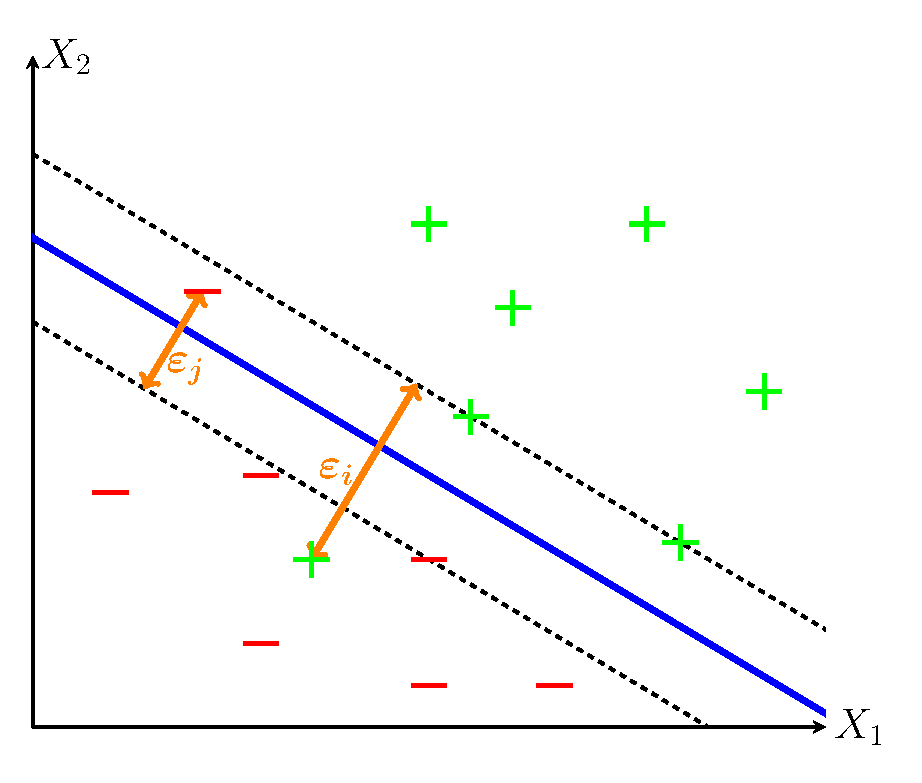
\includegraphics[width=0.5\textwidth,trim=0.5cm 0.5cm 0.5cm 0.5cm]{Images/slackvariable.pdf} 
        \caption{Bedeutung der Slack Variable}
        \label{fig:slackvariable}
\end{figure}

Jetzt könnte man versuchen, diese neue Nebenbedingung einfach in das
zuvor angewandte Optimierungsverfahren einzufügen. Allerdings besteht
hier das Problem, dass \(\varepsilon\) einfach immer maximal groß
gewählt wird und so die Bedingung immer erfüllt wird. Um das Ausmaß der
Verletzung der ursprünglichen Annahmen zu begrenzen, aber trotzdem noch
gewisse Abweichung zuzulassen, wird ein weiterer Parameter \(C\), als
regularisierender Parameter für \(\varepsilon\) eingeführt. Leitet man
daraus zusammen mit der Restriktion \(\varepsilon\ge0\) wieder eine
Lagrangefunktion her erhält man \begin{align}
\mathcal{L}(\overline\beta,\beta_0,\overline\alpha,\overline\varepsilon,\overline\lambda)=\frac{1}{2}\overline\beta'\cdot \overline\beta + C \sum_{i=1}^{n}\varepsilon_i-\underbrace{\sum \alpha_i[y_i(\overline\beta \cdot \overline{x_i}+\beta_0)-1+\varepsilon_i]}_{\text{für }y_i(\overline\beta \cdot \overline{x}_i-\beta_0)>1- \varepsilon_i}-\underbrace{\sum \lambda_i \varepsilon_i }_{\substack{\text{für}\\ \varepsilon_i \ge 0}}
\end{align} Wenn dieser Ausdruck wie beim
\textit{Hard Margin Classifier} gelöst wird und die Ergebnisse
eingesetzt werden erhält man wieder den Ausdruck aus
\eqref{eq:dualproblem} mit der zusätzlichen Einschränkung
\(0\le \alpha_i \le C\) \parencite{bennettSupportVectorMachines2000}.
Diese Min-Max-Optimierung wird dann genauso aufgelöst wie bei dem
\textit{Hard Margin Classifier} und die Entscheidungsregel ist ebenfalls
gleich. Erst durch den Einsatz dieser Technik wurde von der Methode auch
wirklich als \textit{Support Vector Machine} gesprochen
\parencite{vapnikEstimationDependencesBased2006}.

\subsection{Der Kernel Trick}

Auch wenn eine lineare Entscheidungsgrenze Vorteile in Sachen
Generalisierbarkeit bietet, ist sie doch nicht für jede Datensituation
geeignet.In Abbildung \ref{fig:nonlinearsep} ist es sehr gut zu
erkennen, dass in diesem Fall eine lineare Grenze zwischen den Klassen
keinen Sinn ergeben würde und eine elliptische Form wahrscheinlich
besser geeignet wäre. Eine Lösung für dieses Problem, wäre den
Merkmalsraum zu erweitern. So könnte die angenommene Formel für die
lineare Hyperebene in \eqref{eq:hyperebene} durch Polynome der Merkmale
\(X_i\) oder durch Interaktionsterme erweitert werden. Dies führt dazu,
dass die Entscheidungsgrenze in diesem vergrößerten Merkmalsraum immer
noch linear ist, aber die Trennung möglich ist (siehe Abbildung
\ref{fig:featurexten}). Transformiert man diese dann wieder in den
ursprünglichen Merkmalsraum ist die Entscheidungsgrenze dann nicht mehr
linear. Allerdings führt diese Herangehensweise zu einem starken Anstieg
des Rechenaufwands, da die Möglichkeiten der Merkmalserweiterung endlos
sind \parencite{jamesIntroductionStatisticalLearning2021}.

Die Lösung für das Problem sind sogenannte Kernel Funktionen. Betrachtet
man die Entscheidungsfunktion \eqref{eq:decisionf} und setzt für
\(\overline{\beta}\) die Gleichung aus \eqref{eq:solutbeta} erhält man
\begin{align}
f(x_u)= \sum \alpha_i y_i x_i \cdot x_u +\beta_0
\end{align} Es zeigt sich also, dass sich die Entscheidungsfunktion im
Wesentlichen aus einer Linearkombination von Punktprodukten aus dem
Vektor \(x_u\) mit allen Trainingsvektoren \(x_i\) ergibt. Dieses
Punktprodukt kann als Ähnlichkeitsmaß zwischen dem neuen Datenpunkt und
dem jeweiligen Trainingsdatenpunkt interpretiert werden. Es ist nun
möglich diese Produkte durch eine Funktion zu ersetzen, welche die
Ähnlichkeiten von Datenpunkten anders bewertet. Diese sogenannte
\textit{Kernel Funktion} \(K(x_i,x_j)\) ermöglicht es eine flexiblere
Entscheidungsgrenze zu implementieren. Der Vorteil ist dabei, dass die
Kernel Funktion nur auf alle Punktprodukte angewendet wird und es dabei
nicht nötig ist den Merkmalsraum zu erweitern, was wiederum Rechenzeit
spart \parencite{jamesIntroductionStatisticalLearning2021}. Die
Entscheidungsfunktion wird dann mithilfe dieser
\textit{Kernel Funktionen} berechnet: \begin{align}
  f(x_u)=\sum \alpha_i y_i K(x_i,x_u)+\beta_0
\end{align}

\begin{figure}[htb]
    \centering
    \begin{minipage}{0.45\textwidth} 
        \centering
        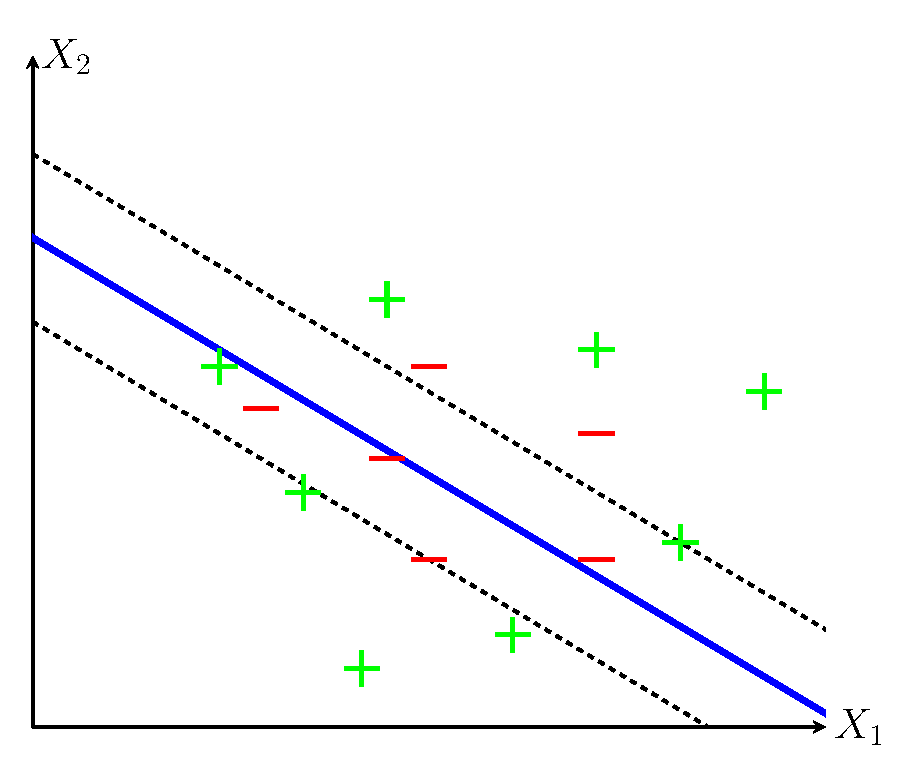
\includegraphics[width=\textwidth,trim=0.5cm 0.5cm 0.5cm 0.5cm]{Images/nonlinearseperable.pdf} 
        \caption{nicht linear getrennte Daten}
        \label{fig:nonlinearsep}
    \end{minipage}\hfill
    \begin{minipage}{0.45\textwidth} 
        \centering
        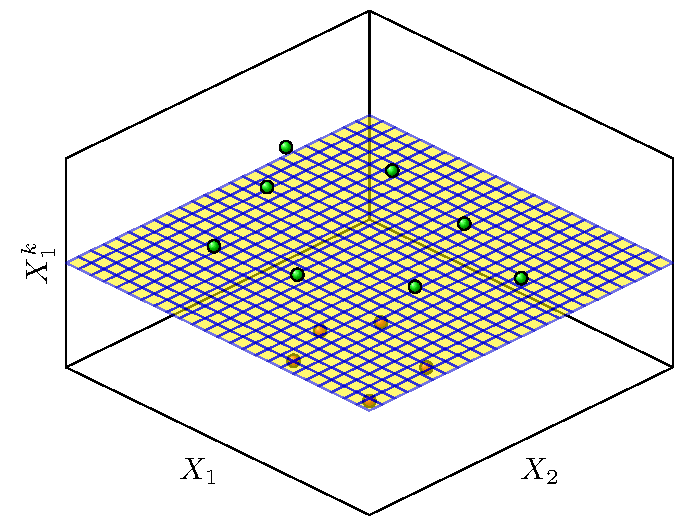
\includegraphics[width=\textwidth,trim=0.5cm 0.5cm 0.5cm 0.5cm]{Images/featurexpansion.pdf}
        \caption{Feature Erweiterung}
        \label{fig:featurexten}
    \end{minipage}
\end{figure}

Es gibt eine ganze Reihe an \textit{Kernel Funktionen}, die bei
\textit{SVM} Anwendung finden. Die Grundlage ist der lineare Kernel,
wobei dieser lediglich das Punktprodukt beschreibt, also praktisch genau
das macht, was bei einer linearen Entscheidungsgrenze gemacht wird. Des
Weiteren gibt es den \textit{Polynomial Kernel}. Dieser hat die Form
\begin{align}
 K(x_i,x_u)=(1+x_i\cdot x_u)^d
\end{align} Die Verwendung von diesem Kernel führt dazu, dass die
Entscheidungsgrenze sich ähnlich Verhält, wie als würde man zu Beginn
eine Merkmalserweiterung mit Polynomen vom Grad \(d\) durchführen (siehe
Abbildung \ref{fig:polykernel}. Eine weitere Kernel Funktion ist der
\textit{Radial Basis Function Kernel} (RBF) mit der Form \begin{align}
K(x_i,x_u)=\exp\left(-\gamma ||x_i-x_u||^2\right)
\end{align} Für diesen Kernel wird die quadrierte euklidische Distanz
als Ähnlichkeitsmaß verwendet, was dazu führt, dass diejenigen \(x_i\)
die näher an \(x_u\) liegen, in der Entscheidungsfunktion einen größeren
Einfluss haben. Der Parameter \(\gamma\) legt dann fest, wie stark der
Einfluss der Distanz sein soll. Die Projektion die der Kernel hier macht
ist eine, in einen unendlich großen Merkmalsraum
\parencite{jamesIntroductionStatisticalLearning2021}. Daher könnte man
selbst durch vorheriges Erweitern des Merkmalsraums nicht das Ergebnis
eines RBF Kernel replizieren, daher führt er auch zu einer sehr
flexiblen Entscheidungsgrenze (siehe Abbildung
\ref{fig:radialkernel}).\\

\begin{figure}[htb]
    \centering
    \begin{minipage}{0.45\textwidth} 
        \centering
        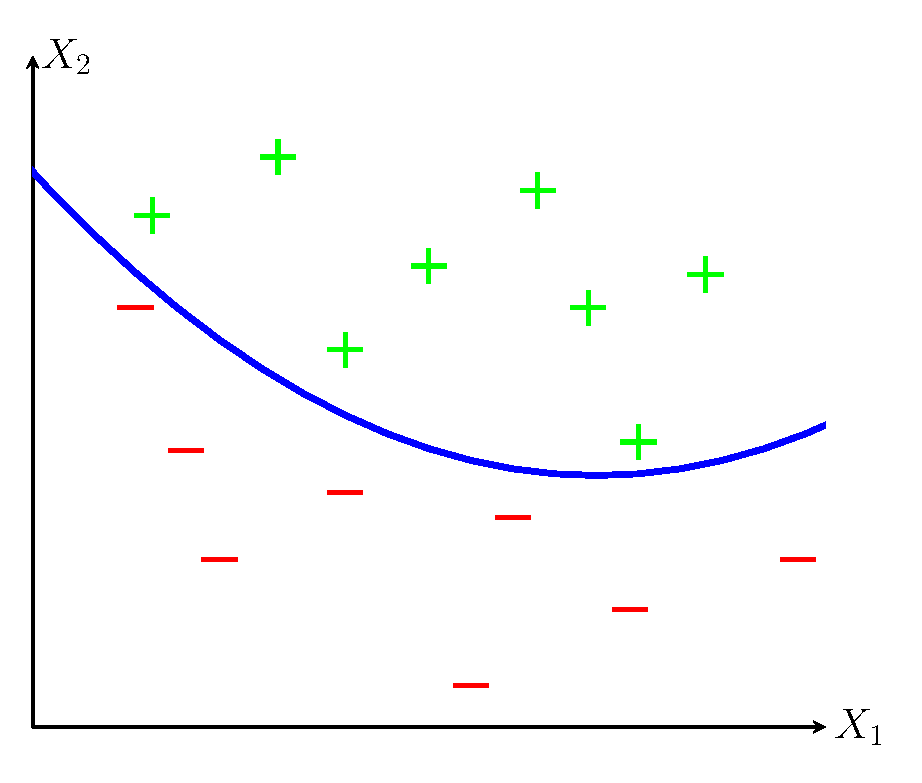
\includegraphics[width=\textwidth,trim=0.5cm 0.5cm 0.5cm 0.5cm]{Images/ploynomial kernel.pdf} 
        \caption{Mögliche Entscheidungsgrenze für polynomial Kernel}
        \label{fig:polykernel}
    \end{minipage}\hfill
    \begin{minipage}{0.45\textwidth} 
        \centering
        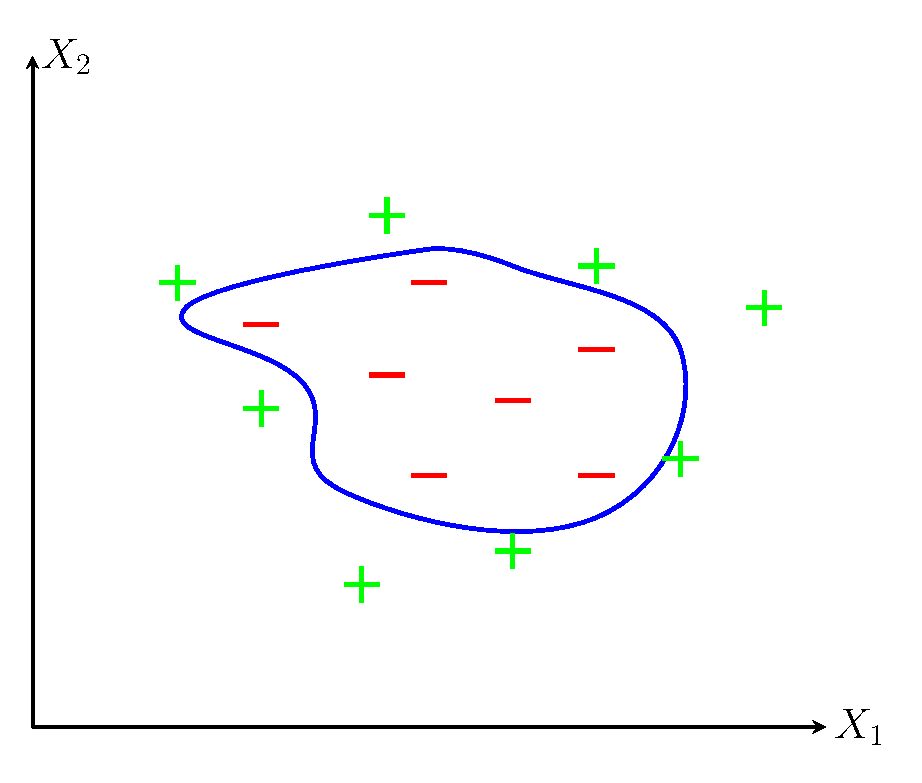
\includegraphics[width=\textwidth,trim=0.5cm 0.5cm 0.5cm 0.5cm]{Images/radial_kernel.pdf}
        \caption{Mögliche Entscheidungsgrenze für RBF Kernel}
        \label{fig:radialkernel}
    \end{minipage}
\end{figure}

Es gibt noch einen Reihe weitere Kernel, die auf unterschiedlichen
Ähnlichkeitsmaßen beruhen, aber eher seltener oder nur in speziellen
Zusammenhänge angewendet werden. Wichtig ist anzumerken, dass die
Verwendung von Kernels zwar die Flexibilität der Entscheidungsgrenze
erhöht, damit aber auch die Gefahr von \textit{Overfitting} einhergeht.
Zusätzlich werden mit den Kernels auch neue Hyperparameter wie \(d\)
oder \(\gamma\) eingeführt, die bei der Modellauswahl ebenfalls beachtet
werden müssen.

\printbibliography

\end{document}
